\documentclass{beamer}

\usetheme{Warsaw}
\setbeamerfont*{frametitle}{size=\normalsize,series=\bfseries}
\setbeamertemplate{navigation symbols}{}
%\usefonttheme{professionalfonts}

\usepackage{listings,bera}
\usepackage[english]{babel}
\usepackage[utf8x]{inputenc}
\usepackage{times}
\usepackage[T1]{fontenc}
\usepackage{ulem}
\usepackage{listings}
\usepackage{textcomp}
\usepackage{graphicx}
\usepackage{subfigure}
\usepackage{hyperref}

%\definecolor{fore}{RGB}{249,242,215}
%\definecolor{back}{RGB}{51,51,51}
%\definecolor{title}{RGB}{255,0,90}
%\setbeamercolor{titlelike}{fg=title}
%\setbeamercolor{normal text}{fg=fore,bg=back}

\definecolor{keywords}{RGB}{255,0,90}
\definecolor{comments}{RGB}{60,179,113}
\definecolor{strings}{RGB}{60,179,60}
\definecolor{numbers}{RGB}{179,60,60}
\lstset{language=Python,
        %extendedchars=false,
        keywordstyle=\color{keywords},
        commentstyle=\color{comments}\emph,
        stringstyle=\color{strings},
        escapechar=!
        }

% adds the \MongoLogo command to put the logo on a slide
\usepackage[absolute,overlay]{textpos}
\setlength{\TPHorizModule}{1mm}
\setlength{\TPVertModule}{1mm}
\newcommand{\MongoLogo}{
\begin{textblock}{14}(2.0,0.7)
  
\includegraphics[height=0.8cm]{logo-mongodb-ondark.png}
\end{textblock}
}

\pgfdeclareimage[height=2in]{featuregraph}{featuresPerformance.png}
\pgfdeclareimage[height=2.5in]{sharding}{sharding.png}

\title{MongoDB}
\subtitle{The new M in the LAMP stack}
\author{Mathias Stearn \\ @mathias\_mongo \\ @mongodb}
\institute{ 
\includegraphics[height=0.8cm]{10gen.png} }
\date{LinuxTag -- 11 June 2010}

%\AtBeginSection[]
%{
  %\begin{frame}<beamer>{}
    %\MongoLogo
    %\tableofcontents[currentsection]
  %\end{frame}
%}


\begin{document}

\begin{frame}
  \MongoLogo
  \titlepage
  
  \begin{center}
    Find this presentation at bit.ly/mongodb-linuxtag
  \end{center}
\end{frame}

%\begin{frame}
  %\MongoLogo
  %\tableofcontents
%\end{frame}

\section{Intro}

\begin{frame}
  \MongoLogo

  \begin{center}
    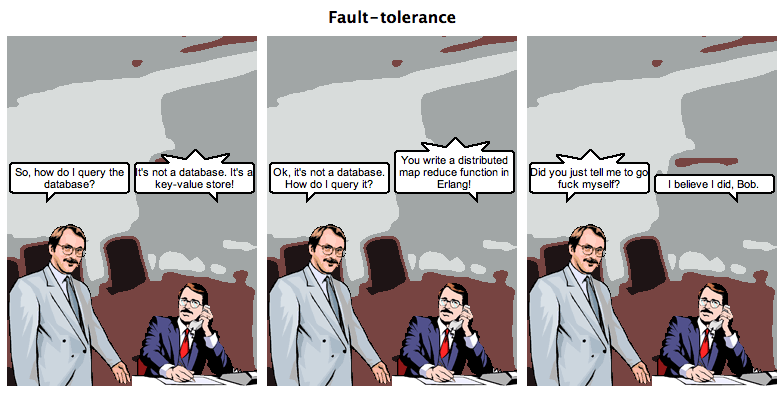
\includegraphics[height=5.5cm]{comic-not-a-db.png} 

    http://browsertoolkit.com/fault-tolerance.png
  \end{center}
\end{frame}

\begin{frame}[fragile]{What is MongoDB?}
  \MongoLogo
  \begin{block}{From http://mongodb.org}
    MongoDB (from ``humongous'') is a scalable, high-performance, open source, document-oriented database
  \end{block}

  In other words, a non-relational database for the masses
\end{frame}

\section{Features for Ops Guys}

\begin{frame}[fragile]{General}
  \MongoLogo
  \begin{itemize}
    \item High performance with large data sets
      \begin{itemize}
        \item Wordnik.com has 1.5TB in over 5 Billion docs
        \item Sustained 100,000 inserts per second during loading
        \item Sustained 250,000 fetches per second during testing
        \item Production Queries are 4x faster than old MySQL setup
      \end{itemize}

    \item Less knobs that need tweaking
    \item Monitoring plugins for Munin, Ganglia, Nagios, and Cacti
    \item Background index building and object removal
    \item 24/7 Support for when you get that 2:00 call

  \end{itemize}
\end{frame}

\begin{frame}[fragile]{Backup}
  \MongoLogo

  \begin{itemize}
    \item $mongodump$ for live backup
    \item $mongoexport$ for JSON dump
    \item fsync-lock command for FS-level snapshots
      \begin{itemize}
        \item Best used with LVM/EBS snaphots
        \item But also works with $tar$ and $rsync$
        \item Can continue reading while locked
      \end{itemize}
  \end{itemize}
\end{frame}

\begin{frame}[fragile]{Replication}
  \MongoLogo

  \begin{itemize}
      \item Very easy to set up
      \item Works across data-centers
      \item Automatic fail-over
        \begin{itemize}
          \item Replica Pairs (Depricated)
          \item Replica Sets (Coming in 1.6)
        \end{itemize}
      \item Slaves do an initial sync then pull operations
      \item Initial sync can be skipped if starting from snapshot
      \item Delayed Replication for ``Oh Schei\ss{}e!'' moments.
  \end{itemize}
\end{frame}


\begin{frame}[fragile]{Sharding: Details}
  \MongoLogo
  \begin{itemize}
    \item No single point of failure
    \item Automatic range-based partitioning
    \item You app connects to a $mongos$ rather than a $mongod$
    \item You pick which collections are sharded
    \item You pick a shard-key for those collections
    \item No other changes are necessary in your app
    \item We handle the rest!
  \end{itemize}
\end{frame}

\begin{frame}
  \MongoLogo
  \center
  \pgfuseimage{sharding}
\end{frame}

\section{Features for Devs}

\begin{frame}[fragile]{Inserting}
  \MongoLogo

\begin{lstlisting}
db.posts.insert( {
    by: 'mstearn',
    posted: Date(12345),
    text: 'Mongo is Better than Your Database',
    tags: ['MongoDB', '#win'],
    votes: 100,
    comments: [
        { by: 'joe_schmoe',
          text: 'Why?',
          votes: 10 }
    ]
})
\end{lstlisting}
\end{frame}

\begin{frame}[fragile]
  \MongoLogo

  \begin{lstlisting}
db.posts.find({by: 'mstearn'})
db.posts.find({by: 'mstearn'}).sort({posted:-1})
db.posts.find({'comments.by': 'joe_schmoe'})

db.posts.find().sort({votes: -1}).limit(10)
db.posts.find({votes: {$gte: 40, $lt: 50}}) 

db.posts.find({text: /mongodb/i})

db.posts.ensureIndex({tags: 1})
db.posts.find({tags: 'MongoDB'})
db.posts.find({tags: {$in:['MongoDB', 'MySQL']}})
db.posts.find({tags: {$all:['MongoDB', 'MySQL']}})
  \end{lstlisting}
\end{frame}

\begin{frame}[fragile]{Pretty Python Queries with MongoMagic}
  \MongoLogo

  \begin{block}{Shameless self-promotion}
    \url{http://github.com/RedBeard0531/MongoMagic/}
  \end{block}

  \begin{lstlisting}
db.posts.find( M.by == 'mstearn' )
db.posts.find( 40 <= M.votes < 50 ) 
db.posts.find( M.comments.by == 'joe_schmoe' )
db.posts.find( M.tags.IN('MongoDB', 'MySQL') )
  \end{lstlisting}
\end{frame}

\begin{frame}[fragile]{2D Geospatial Queries}
  \MongoLogo

  \small
  \begin{lstlisting}
db.zips.insert({_id: '10011', loc: [43, -74]})

db.zips.ensureIndex({loc: '2d'})

db.zips.find({loc: {$near: [43, -74]}})

var box = [[x1, y1], [x2, y2]]
db.zips.find({loc: {$within: {$box: box}}})

var circle = [[x,y], radius]
db.zips.find({loc: {$within: {$center: circle}}})
                 
  \end{lstlisting}
\end{frame}

\begin{frame}
  \MongoLogo

  \center {\huge Questions?}

  \begin{block}{Links}
  \begin{itemize}
    \item http://bit.ly/mongodb-linuxtag
    \item http://github.com/RedBeard0531/MongoMagic
    \item http://try.mongodb.org (Try mongo in your browser)
    \item http://www.mongodb.org
    \item \#mongodb on irc.freenode.net
    \item mongodb-user on google groups
  \end{itemize}
  \end{block}

  \begin{block}{Contact}
  \begin{itemize}
    \item mathias@10gen.com
    \item @mathias\_mongo ${\leftarrow}$ follow me!
  \end{itemize}
  \end{block}
\end{frame}

\end{document}

% vim: set softtabstop=2
